% Options for packages loaded elsewhere
\PassOptionsToPackage{unicode}{hyperref}
\PassOptionsToPackage{hyphens}{url}
%
\documentclass[
]{article}
\usepackage{lmodern}
\usepackage{amssymb,amsmath}
\usepackage{ifxetex,ifluatex}
\ifnum 0\ifxetex 1\fi\ifluatex 1\fi=0 % if pdftex
  \usepackage[T1]{fontenc}
  \usepackage[utf8]{inputenc}
  \usepackage{textcomp} % provide euro and other symbols
\else % if luatex or xetex
  \usepackage{unicode-math}
  \defaultfontfeatures{Scale=MatchLowercase}
  \defaultfontfeatures[\rmfamily]{Ligatures=TeX,Scale=1}
\fi
% Use upquote if available, for straight quotes in verbatim environments
\IfFileExists{upquote.sty}{\usepackage{upquote}}{}
\IfFileExists{microtype.sty}{% use microtype if available
  \usepackage[]{microtype}
  \UseMicrotypeSet[protrusion]{basicmath} % disable protrusion for tt fonts
}{}
\makeatletter
\@ifundefined{KOMAClassName}{% if non-KOMA class
  \IfFileExists{parskip.sty}{%
    \usepackage{parskip}
  }{% else
    \setlength{\parindent}{0pt}
    \setlength{\parskip}{6pt plus 2pt minus 1pt}}
}{% if KOMA class
  \KOMAoptions{parskip=half}}
\makeatother
\usepackage{xcolor}
\IfFileExists{xurl.sty}{\usepackage{xurl}}{} % add URL line breaks if available
\IfFileExists{bookmark.sty}{\usepackage{bookmark}}{\usepackage{hyperref}}
\hypersetup{
  pdftitle={What you can and can't do to change your grades},
  pdfauthor={Laine Wishart and Asela Gunatilake},
  hidelinks,
  pdfcreator={LaTeX via pandoc}}
\urlstyle{same} % disable monospaced font for URLs
\usepackage[margin=1in]{geometry}
\usepackage{color}
\usepackage{fancyvrb}
\newcommand{\VerbBar}{|}
\newcommand{\VERB}{\Verb[commandchars=\\\{\}]}
\DefineVerbatimEnvironment{Highlighting}{Verbatim}{commandchars=\\\{\}}
% Add ',fontsize=\small' for more characters per line
\usepackage{framed}
\definecolor{shadecolor}{RGB}{248,248,248}
\newenvironment{Shaded}{\begin{snugshade}}{\end{snugshade}}
\newcommand{\AlertTok}[1]{\textcolor[rgb]{0.94,0.16,0.16}{#1}}
\newcommand{\AnnotationTok}[1]{\textcolor[rgb]{0.56,0.35,0.01}{\textbf{\textit{#1}}}}
\newcommand{\AttributeTok}[1]{\textcolor[rgb]{0.77,0.63,0.00}{#1}}
\newcommand{\BaseNTok}[1]{\textcolor[rgb]{0.00,0.00,0.81}{#1}}
\newcommand{\BuiltInTok}[1]{#1}
\newcommand{\CharTok}[1]{\textcolor[rgb]{0.31,0.60,0.02}{#1}}
\newcommand{\CommentTok}[1]{\textcolor[rgb]{0.56,0.35,0.01}{\textit{#1}}}
\newcommand{\CommentVarTok}[1]{\textcolor[rgb]{0.56,0.35,0.01}{\textbf{\textit{#1}}}}
\newcommand{\ConstantTok}[1]{\textcolor[rgb]{0.00,0.00,0.00}{#1}}
\newcommand{\ControlFlowTok}[1]{\textcolor[rgb]{0.13,0.29,0.53}{\textbf{#1}}}
\newcommand{\DataTypeTok}[1]{\textcolor[rgb]{0.13,0.29,0.53}{#1}}
\newcommand{\DecValTok}[1]{\textcolor[rgb]{0.00,0.00,0.81}{#1}}
\newcommand{\DocumentationTok}[1]{\textcolor[rgb]{0.56,0.35,0.01}{\textbf{\textit{#1}}}}
\newcommand{\ErrorTok}[1]{\textcolor[rgb]{0.64,0.00,0.00}{\textbf{#1}}}
\newcommand{\ExtensionTok}[1]{#1}
\newcommand{\FloatTok}[1]{\textcolor[rgb]{0.00,0.00,0.81}{#1}}
\newcommand{\FunctionTok}[1]{\textcolor[rgb]{0.00,0.00,0.00}{#1}}
\newcommand{\ImportTok}[1]{#1}
\newcommand{\InformationTok}[1]{\textcolor[rgb]{0.56,0.35,0.01}{\textbf{\textit{#1}}}}
\newcommand{\KeywordTok}[1]{\textcolor[rgb]{0.13,0.29,0.53}{\textbf{#1}}}
\newcommand{\NormalTok}[1]{#1}
\newcommand{\OperatorTok}[1]{\textcolor[rgb]{0.81,0.36,0.00}{\textbf{#1}}}
\newcommand{\OtherTok}[1]{\textcolor[rgb]{0.56,0.35,0.01}{#1}}
\newcommand{\PreprocessorTok}[1]{\textcolor[rgb]{0.56,0.35,0.01}{\textit{#1}}}
\newcommand{\RegionMarkerTok}[1]{#1}
\newcommand{\SpecialCharTok}[1]{\textcolor[rgb]{0.00,0.00,0.00}{#1}}
\newcommand{\SpecialStringTok}[1]{\textcolor[rgb]{0.31,0.60,0.02}{#1}}
\newcommand{\StringTok}[1]{\textcolor[rgb]{0.31,0.60,0.02}{#1}}
\newcommand{\VariableTok}[1]{\textcolor[rgb]{0.00,0.00,0.00}{#1}}
\newcommand{\VerbatimStringTok}[1]{\textcolor[rgb]{0.31,0.60,0.02}{#1}}
\newcommand{\WarningTok}[1]{\textcolor[rgb]{0.56,0.35,0.01}{\textbf{\textit{#1}}}}
\usepackage{graphicx,grffile}
\makeatletter
\def\maxwidth{\ifdim\Gin@nat@width>\linewidth\linewidth\else\Gin@nat@width\fi}
\def\maxheight{\ifdim\Gin@nat@height>\textheight\textheight\else\Gin@nat@height\fi}
\makeatother
% Scale images if necessary, so that they will not overflow the page
% margins by default, and it is still possible to overwrite the defaults
% using explicit options in \includegraphics[width, height, ...]{}
\setkeys{Gin}{width=\maxwidth,height=\maxheight,keepaspectratio}
% Set default figure placement to htbp
\makeatletter
\def\fps@figure{htbp}
\makeatother
\setlength{\emergencystretch}{3em} % prevent overfull lines
\providecommand{\tightlist}{%
  \setlength{\itemsep}{0pt}\setlength{\parskip}{0pt}}
\setcounter{secnumdepth}{-\maxdimen} % remove section numbering

\title{What you can and can't do to change your grades}
\author{Laine Wishart and Asela Gunatilake}
\date{11/04/2021}

\begin{document}
\maketitle

\begin{Shaded}
\begin{Highlighting}[]
\KeywordTok{library}\NormalTok{(ggplot2)}
\KeywordTok{library}\NormalTok{(caret)}
\KeywordTok{library}\NormalTok{(tidyverse)}
\KeywordTok{library}\NormalTok{(dplyr)}
\KeywordTok{library}\NormalTok{(janitor)}
\end{Highlighting}
\end{Shaded}

\begin{Shaded}
\begin{Highlighting}[]
\NormalTok{d.mat=}\KeywordTok{read.table}\NormalTok{(}\StringTok{"data/student/student-mat.csv"}\NormalTok{,}\DataTypeTok{sep=}\StringTok{";"}\NormalTok{,}\DataTypeTok{header=}\OtherTok{TRUE}\NormalTok{)}
\NormalTok{d.port=}\KeywordTok{read.table}\NormalTok{(}\StringTok{"data/student/student-por.csv"}\NormalTok{,}\DataTypeTok{sep=}\StringTok{";"}\NormalTok{,}\DataTypeTok{header=}\OtherTok{TRUE}\NormalTok{)}
\NormalTok{d.mat}\OperatorTok{$}\NormalTok{subject =}\StringTok{ "Maths"}
\NormalTok{d.port}\OperatorTok{$}\NormalTok{subject =}\StringTok{ "Portugese"}
\NormalTok{d.all <-}\StringTok{ }\KeywordTok{rbind}\NormalTok{(d.mat, d.port) }\CommentTok{#%>% mutate(Medu = as.factor(Medu), }
                 \CommentTok{#studytime = as.factor(studytime))}
\end{Highlighting}
\end{Shaded}

breaking down the factors that influence your grades based on a the
dataset.

In this sample of students, aged between 16 - 22,male female ratio,
attended two schools in Portugal, demographic data were collected among
with scores for Math and Portuguese.

We have divided the attributes based on environmental, non, controllable
factors (e.g.~age, gender, family background) and ``factors that can be
controlled by the student'' xx (e.g.~number of hours spent studying,
frequency of going out, alcohol consumption ). Our analyses indicate
that both factors played a role in determining student grade and may be
transferable to university setting.

More importantly, students who found a \textbf{``goldilocks''} zone
between work and life appeared to perform strongest as a group.

\textbf{top achievers what did they look like???maybe look at the top
5\% and find their attributes???}

\hypertarget{family-influence-on-student-achievement}{%
\section{Family influence on student
achievement}\label{family-influence-on-student-achievement}}

\hypertarget{but-mothers-education-matters}{%
\section{(but mother's education
matters)}\label{but-mothers-education-matters}}

\begin{center}\rule{0.5\linewidth}{0.5pt}\end{center}

\begin{Shaded}
\begin{Highlighting}[]
\NormalTok{d.all <-}\StringTok{ }\NormalTok{d.all }\OperatorTok\StringTok{ }\KeywordTok{mutate}\NormalTok{(}\DataTypeTok{Medu =} \KeywordTok{case_when}\NormalTok{(Medu }\OperatorTok{==}\StringTok{ }\DecValTok{0} \OperatorTok{~}\StringTok{ "None"}\NormalTok{,}
\NormalTok{                                  Medu }\OperatorTok{==}\StringTok{ }\DecValTok{1} \OperatorTok{~}\StringTok{ "4th Grade"}\NormalTok{, }
\NormalTok{                                  Medu }\OperatorTok{==}\StringTok{ }\DecValTok{2} \OperatorTok{~}\StringTok{ "5th - 9th Grade"}\NormalTok{, }
\NormalTok{                                  Medu }\OperatorTok{==}\StringTok{ }\DecValTok{3} \OperatorTok{~}\StringTok{ "Secondary Education"}\NormalTok{, }
\NormalTok{                                  Medu }\OperatorTok{==}\StringTok{ }\DecValTok{4} \OperatorTok{~}\StringTok{ "Higher Education"}\NormalTok{))}


\NormalTok{d.all}\OperatorTok{$}\NormalTok{Medu =}\StringTok{ }\KeywordTok{factor}\NormalTok{(d.all}\OperatorTok{$}\NormalTok{Medu, }\DataTypeTok{levels =}  \KeywordTok{c}\NormalTok{(}\StringTok{"None"}\NormalTok{, }\StringTok{"4th Grade"}\NormalTok{, }\StringTok{"5th - 9th Grade"}\NormalTok{,  }\StringTok{"Secondary Education"}\NormalTok{, }\StringTok{"Higher Education"}\NormalTok{), }\DataTypeTok{ordered =} \OtherTok{TRUE}\NormalTok{ )}
\CommentTok{#levels(d.all$Medu) = c("None", "4th Grade", "5th - 9th Grade",  "Secondary Education", "Higher #Education")}

\NormalTok{d.all }\OperatorTok\StringTok{ }
\StringTok{  }\KeywordTok{ggplot}\NormalTok{(}\KeywordTok{aes}\NormalTok{(}\DataTypeTok{x =}\NormalTok{ Medu, }\DataTypeTok{y =}\NormalTok{ G3, }\DataTypeTok{fill =}\NormalTok{ subject)) }\OperatorTok{+}\StringTok{ }\KeywordTok{geom_boxplot}\NormalTok{() }\OperatorTok{+}\StringTok{ }\KeywordTok{labs}\NormalTok{(}\DataTypeTok{title =} \StringTok{"Student performance by mother's education level"}\NormalTok{, }\DataTypeTok{x =} \StringTok{"Mother's education level"}\NormalTok{, }\DataTypeTok{y =} \StringTok{"Student performane"}\NormalTok{, }\DataTypeTok{fill =} \StringTok{"Subject"}\NormalTok{) }\OperatorTok{+}\StringTok{ }\KeywordTok{theme_bw}\NormalTok{() }\OperatorTok{+}\StringTok{ }\KeywordTok{theme}\NormalTok{(}\DataTypeTok{axis.text.x =} \KeywordTok{element_text}\NormalTok{(}\DataTypeTok{angle =} \DecValTok{45}\NormalTok{, }\DataTypeTok{hjust=}\DecValTok{1}\NormalTok{))}
\end{Highlighting}
\end{Shaded}

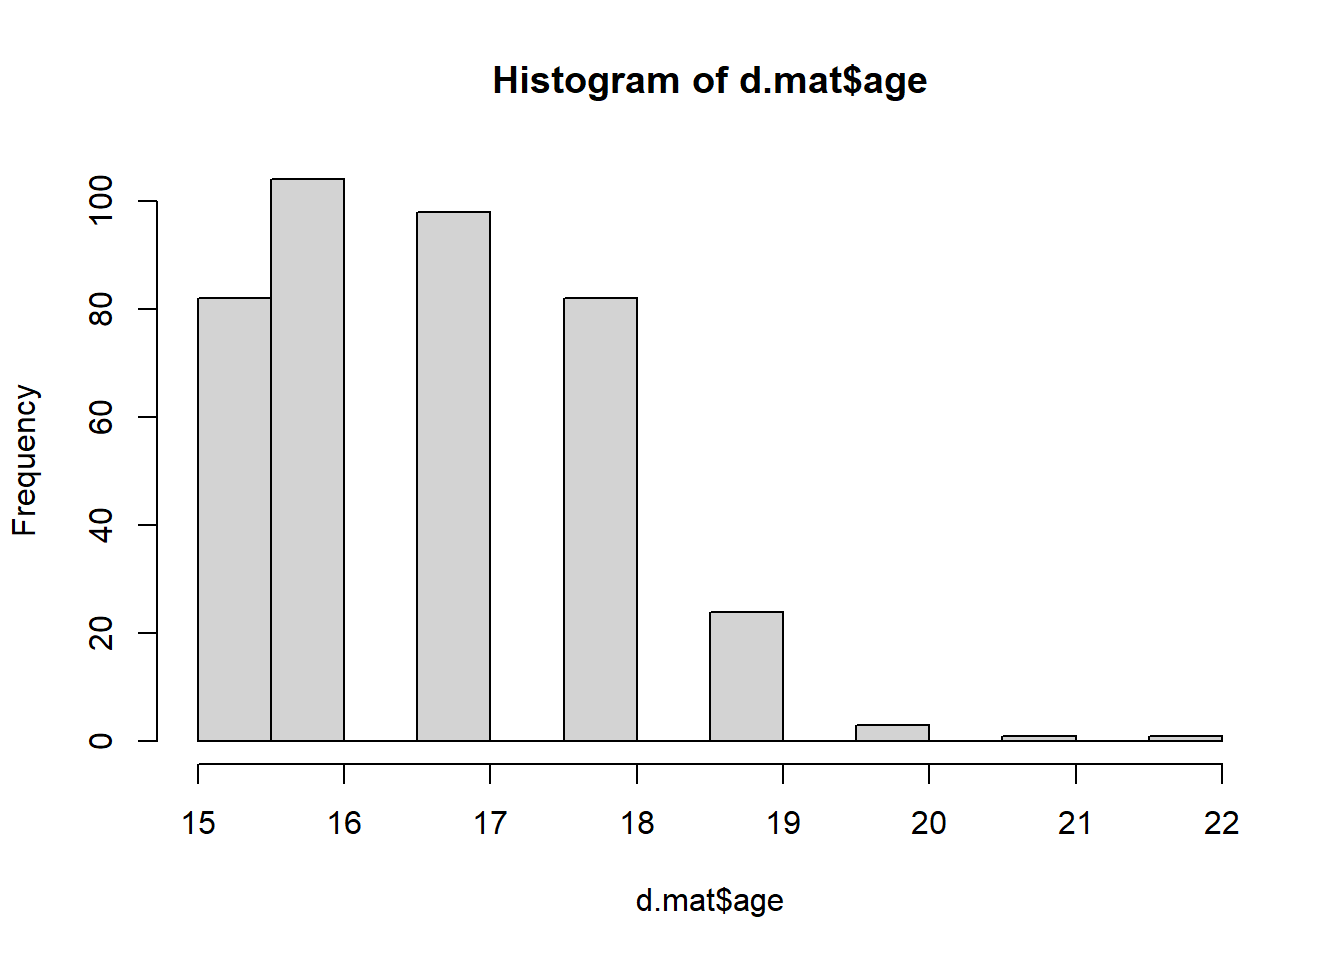
\includegraphics{journal-article_files/figure-latex/unnamed-chunk-3-1.pdf}

In this study, a student's mark in both Portugese and Math increased
positively with his mother's and father's education level. As shown in
the figure above, when mothers have a low education level, their
children perform poorly compared to their peers. One study in 2015
explored how parent-education levels affected student engagement in
school over a period of several years in Japan (Matsuoka et al., 2015).
They found that a parent's education level influenced their parenting
style: highly-educated parents tend to schedule their children's time
with more extracurricular activities, and place a larger emphasis on
engaging language to reason. Educated parents may also have higher
expectations for their children's academic achievement, which could
subsequently influence their desires to pursue higher education: one
study found that the mother's expectations for her children had an
impact on whether they wanted to attend university (Uzuki, 2004).

\begin{Shaded}
\begin{Highlighting}[]
\NormalTok{d.all }\OperatorTok\StringTok{ }\KeywordTok{ggplot}\NormalTok{(}\KeywordTok{aes}\NormalTok{(}\DataTypeTok{x =}\NormalTok{ Medu, }\DataTypeTok{y =}\NormalTok{ G3, }\DataTypeTok{fill =}\NormalTok{ studytime)) }\OperatorTok{+}\StringTok{ }\KeywordTok{geom_boxplot}\NormalTok{() }\OperatorTok{+}\StringTok{ }\KeywordTok{labs}\NormalTok{(}\DataTypeTok{title =} \StringTok{"Student performance by mother's education level"}\NormalTok{, }\DataTypeTok{x =} \StringTok{"Mother's education level"}\NormalTok{, }\DataTypeTok{y =} \StringTok{"Student performane"}\NormalTok{, }\DataTypeTok{fill =} \StringTok{"Study time (hours)"}\NormalTok{) }\OperatorTok{+}\StringTok{ }\KeywordTok{theme_bw}\NormalTok{() }\OperatorTok{+}\StringTok{ }\KeywordTok{facet_wrap}\NormalTok{(}\OperatorTok{~}\NormalTok{subject, }\DataTypeTok{nrow =} \DecValTok{2}\NormalTok{) }\OperatorTok{+}\StringTok{ }\KeywordTok{theme}\NormalTok{(}\DataTypeTok{axis.text.x =} \KeywordTok{element_text}\NormalTok{(}\DataTypeTok{angle =} \DecValTok{45}\NormalTok{, }\DataTypeTok{hjust=}\DecValTok{1}\NormalTok{))}
\end{Highlighting}
\end{Shaded}

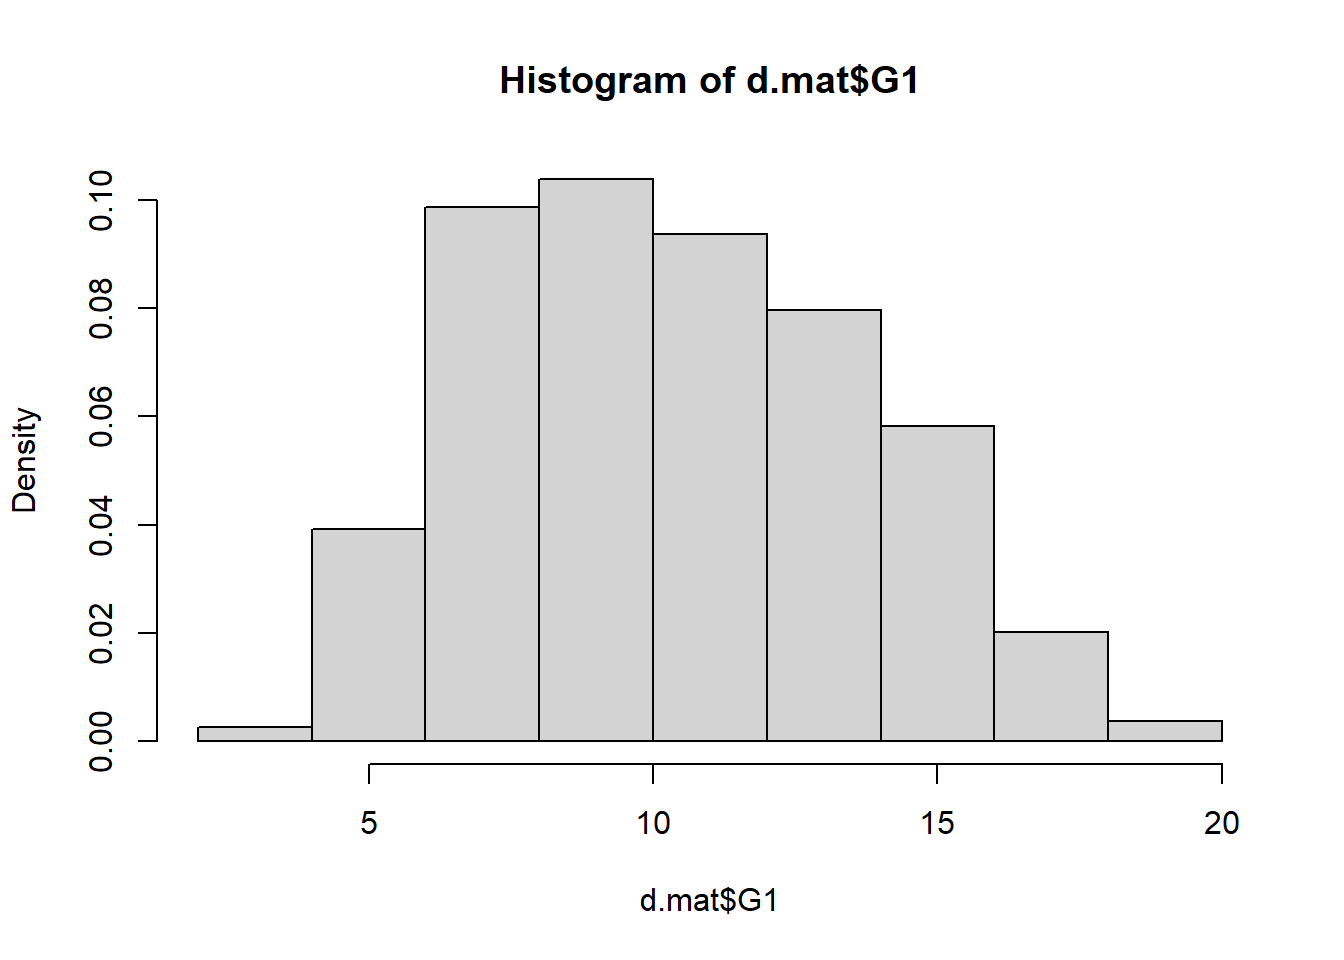
\includegraphics{journal-article_files/figure-latex/unnamed-chunk-4-1.pdf}

Although parent education appears to affect how students spend their
free time and shape their future academic goals, individual effort
appears to pay off more for students from poorly-educated families. The
above figure shows there was a larger increase in sacacemic achievement
per increase in hours studies for students with poorly-educated mothers
compared to students with highly educated mothers.

\hypertarget{student-choices-on-student-achievement}{%
\section{Student choices on student
achievement}\label{student-choices-on-student-achievement}}

\begin{center}\rule{0.5\linewidth}{0.5pt}\end{center}

Important to note the balance between

The dataset has

\hypertarget{the-amount-of-hours-you-study-translates-to-higher-marks-but-at-a-diminishing-rate}{%
\subsection{The amount of hours you study translates to higher marks,
but at a diminishing
rate}\label{the-amount-of-hours-you-study-translates-to-higher-marks-but-at-a-diminishing-rate}}

\begin{center}\rule{0.5\linewidth}{0.5pt}\end{center}

\begin{Shaded}
\begin{Highlighting}[]
\NormalTok{d.mat}\OperatorTok{$}\NormalTok{G4 <-}\StringTok{ }\NormalTok{(}\FloatTok{0.3}\OperatorTok{*}\NormalTok{d.mat}\OperatorTok{$}\NormalTok{G1 }\OperatorTok{+}\StringTok{ }\FloatTok{0.3}\OperatorTok{*}\NormalTok{d.mat}\OperatorTok{$}\NormalTok{G2 }\OperatorTok{+}\StringTok{ }\FloatTok{0.4}\OperatorTok{*}\NormalTok{d.mat}\OperatorTok{$}\NormalTok{G3)}\OperatorTok{/}\DecValTok{20} 
\NormalTok{d.port}\OperatorTok{$}\NormalTok{G4 <-}\StringTok{ }\NormalTok{(}\FloatTok{0.3}\OperatorTok{*}\NormalTok{d.port}\OperatorTok{$}\NormalTok{G1 }\OperatorTok{+}\StringTok{ }\FloatTok{0.3}\OperatorTok{*}\NormalTok{d.port}\OperatorTok{$}\NormalTok{G2 }\OperatorTok{+}\StringTok{ }\FloatTok{0.4}\OperatorTok{*}\NormalTok{d.port}\OperatorTok{$}\NormalTok{G3)}\OperatorTok{/}\DecValTok{20} 


\NormalTok{d.all <-}\StringTok{ }\NormalTok{d.all }\OperatorTok\StringTok{ }\KeywordTok{mutate}\NormalTok{(}\DataTypeTok{studytime =} \KeywordTok{case_when}\NormalTok{(studytime }\OperatorTok{==}\StringTok{ }\DecValTok{1} \OperatorTok{~}\StringTok{ "[1-2)"}\NormalTok{,}
\NormalTok{                                       studytime }\OperatorTok{==}\StringTok{ }\DecValTok{2} \OperatorTok{~}\StringTok{ "[2-5)"}\NormalTok{, }
\NormalTok{                                       studytime }\OperatorTok{==}\StringTok{ }\DecValTok{3} \OperatorTok{~}\StringTok{ "[3-10)"}\NormalTok{, }
\NormalTok{                                       studytime }\OperatorTok{==}\StringTok{ }\DecValTok{4}\OperatorTok{~}\StringTok{ "[4-10)"}\NormalTok{)) }

\NormalTok{d.all }\OperatorTok\StringTok{ }\KeywordTok{ggplot}\NormalTok{(}\KeywordTok{aes}\NormalTok{(}\DataTypeTok{x =}\NormalTok{ studytime, }\DataTypeTok{y =}\NormalTok{ G3, }\DataTypeTok{fill =}\NormalTok{ subject)) }\OperatorTok{+}\StringTok{ }\KeywordTok{geom_boxplot}\NormalTok{() }\OperatorTok{+}\StringTok{ }\KeywordTok{labs}\NormalTok{( }\DataTypeTok{title =} \StringTok{"Academic performance by study time"}\NormalTok{, }\DataTypeTok{x =} \StringTok{"Study time (hours)"}\NormalTok{, }\DataTypeTok{y =} \StringTok{"Academic performance"}\NormalTok{) }\OperatorTok{+}\StringTok{ }\KeywordTok{theme_bw}\NormalTok{() }
\end{Highlighting}
\end{Shaded}

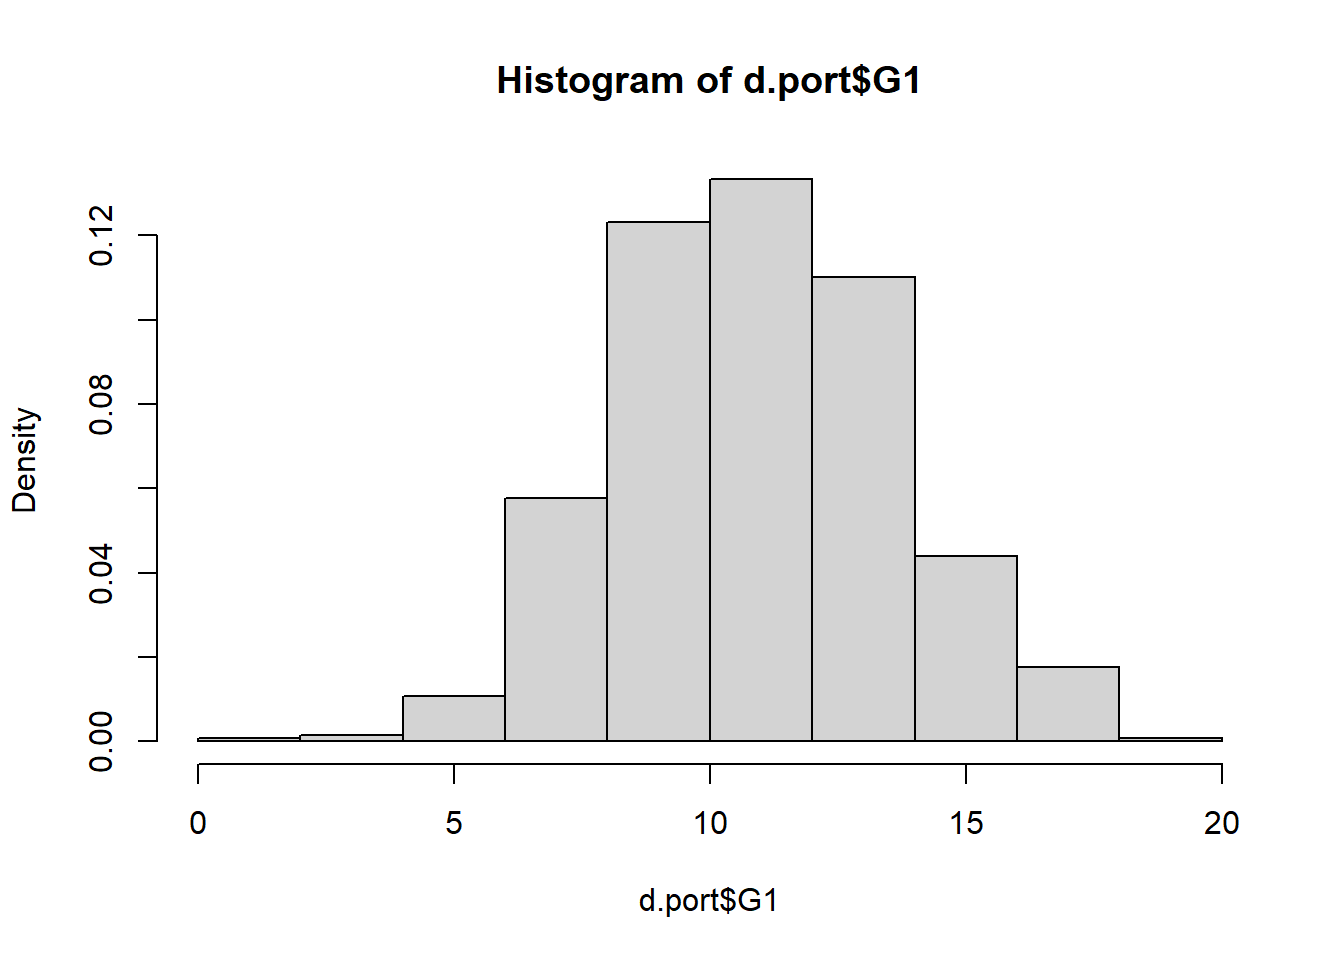
\includegraphics{journal-article_files/figure-latex/unnamed-chunk-5-1.pdf}

In most cases, students who studied more hours per week were able to
transfer their effort in to better grades albeit at a diminishing rate.
However, it appears the scores deteriorated for the cohort of students
that studied more than 10 hours per week relative to the cohort of
students who reportedly studied between 5 to 10 hours per week. This may
be indicative of additional studying time infringing on students'
free-time and the ability to engage in social activities. As we explore
in the subsequent chapters, \emph{``all-work no play''} strategy may not
neccasarly equates to gains in grades.

\hypertarget{not-having-free-time-is-expensive-having-too-much-of-it-is-not-good-either}{%
\subsection{Not having free time is expensive, having too much of it is
not good
either}\label{not-having-free-time-is-expensive-having-too-much-of-it-is-not-good-either}}

\begin{center}\rule{0.5\linewidth}{0.5pt}\end{center}

\begin{Shaded}
\begin{Highlighting}[]
\NormalTok{d.all <-}\StringTok{ }\NormalTok{d.all }\OperatorTok\StringTok{ }\KeywordTok{mutate}\NormalTok{(}\DataTypeTok{freetime =} \KeywordTok{case_when}\NormalTok{(}
\NormalTok{  freetime }\OperatorTok{==}\StringTok{ }\DecValTok{1} \OperatorTok{~}\StringTok{ "Very Low"}\NormalTok{, }
\NormalTok{  freetime }\OperatorTok{==}\StringTok{ }\DecValTok{2} \OperatorTok{~}\StringTok{ "Low"}\NormalTok{, }
\NormalTok{  freetime }\OperatorTok{==}\StringTok{ }\DecValTok{3} \OperatorTok{~}\StringTok{ "Average"}\NormalTok{, }
\NormalTok{  freetime }\OperatorTok{==}\StringTok{ }\DecValTok{4} \OperatorTok{~}\StringTok{ "High"}\NormalTok{,}
\NormalTok{  freetime }\OperatorTok{==}\StringTok{ }\DecValTok{5} \OperatorTok{~}\StringTok{ "Very High"}
\NormalTok{))}

\NormalTok{d.all}\OperatorTok{$}\NormalTok{freetime =}\StringTok{ }\KeywordTok{factor}\NormalTok{(d.all}\OperatorTok{$}\NormalTok{freetime, }\DataTypeTok{levels =} \KeywordTok{c}\NormalTok{(}\StringTok{"Very Low"}\NormalTok{,}\StringTok{"Low"}\NormalTok{,}\StringTok{"Average"}\NormalTok{,}\StringTok{"High"}\NormalTok{,}\StringTok{'Very High'}\NormalTok{), }\DataTypeTok{ordered=}\OtherTok{TRUE}\NormalTok{)}
\NormalTok{d.all }\OperatorTok\StringTok{ }\KeywordTok{ggplot}\NormalTok{(}\KeywordTok{aes}\NormalTok{(}\DataTypeTok{x =}\NormalTok{ freetime, }\DataTypeTok{y =}\NormalTok{ G3)) }\OperatorTok{+}\StringTok{ }\KeywordTok{geom_boxplot}\NormalTok{() }\OperatorTok{+}\StringTok{ }\KeywordTok{labs}\NormalTok{(}\DataTypeTok{title =} \StringTok{"Academic performance by free time after school"}\NormalTok{, }\DataTypeTok{x =} \StringTok{""}\NormalTok{, }\DataTypeTok{y =} \StringTok{"Academic performance"}\NormalTok{) }\OperatorTok{+}\StringTok{ }\KeywordTok{theme_bw}\NormalTok{() }\OperatorTok{+}\StringTok{ }\KeywordTok{facet_wrap}\NormalTok{(}\OperatorTok{~}\StringTok{ }\NormalTok{subject, }\DataTypeTok{nrow =} \DecValTok{1}\NormalTok{)}
\end{Highlighting}
\end{Shaded}

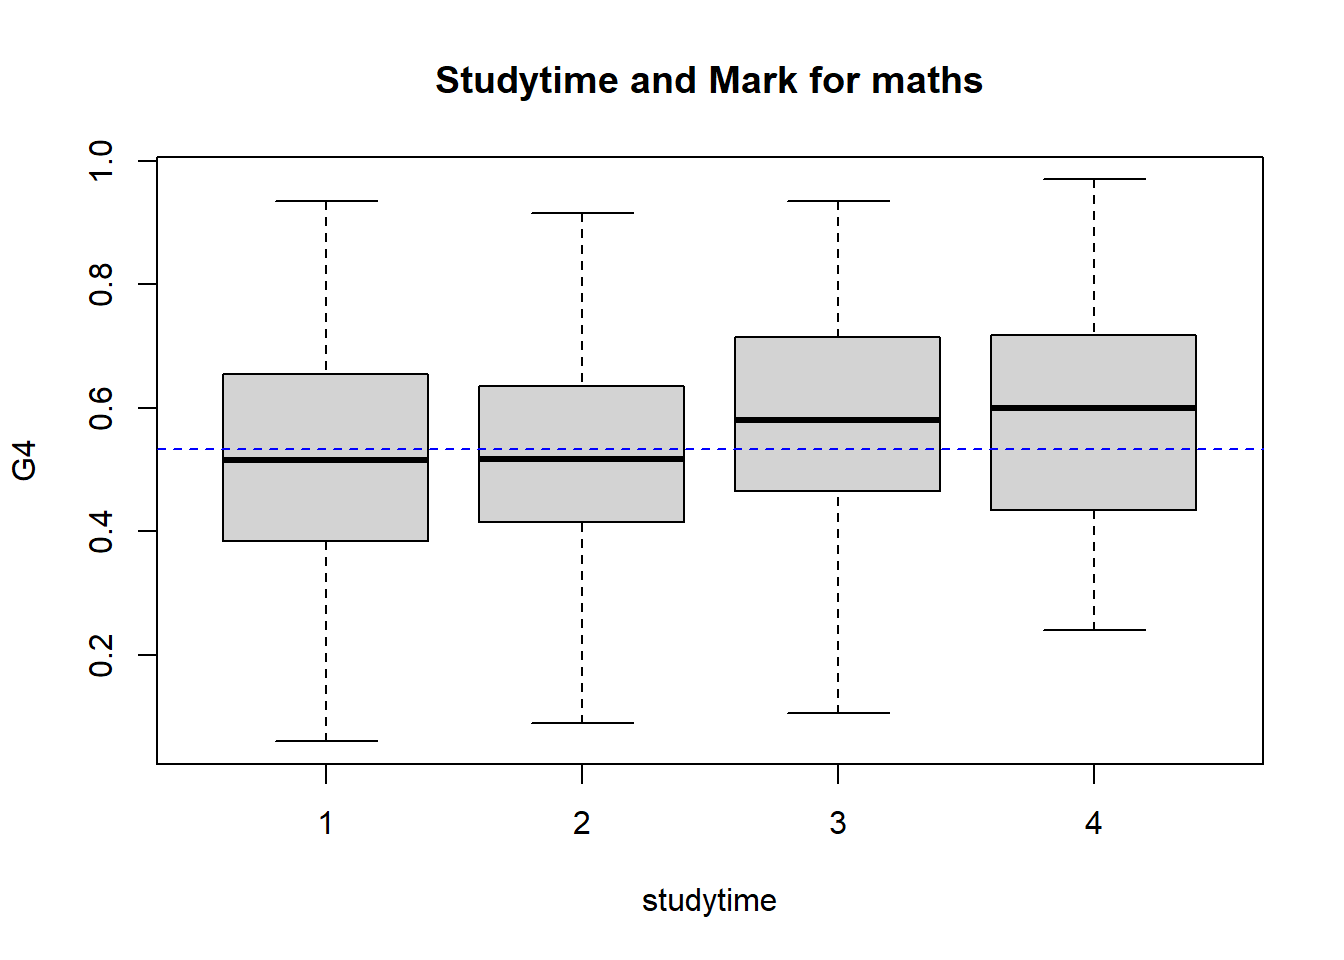
\includegraphics{journal-article_files/figure-latex/unnamed-chunk-6-1.pdf}

The results based on the sample of 365 students, shows that having very
little free time and having too much free time can both result in lower
grades. This result is more pronounced in language test results.
However, for both math and language a \emph{``goldilocks''} zone of
``free time'' appears to correspond with the cohort of strongest
academic achievers. This result is inline with the conventional wisdom
that achieving a optimal \emph{``work live balance''} is beneficial for
academic accomplishment.

\hypertarget{finding-the-sweetspot-in-going-out}{%
\subsection{Finding the sweetspot in going
out}\label{finding-the-sweetspot-in-going-out}}

\begin{center}\rule{0.5\linewidth}{0.5pt}\end{center}

\begin{Shaded}
\begin{Highlighting}[]
\NormalTok{d.all <-}\StringTok{ }\NormalTok{d.all }\OperatorTok\StringTok{ }\KeywordTok{mutate}\NormalTok{(}\DataTypeTok{goout =} \KeywordTok{case_when}\NormalTok{(}
\NormalTok{  goout }\OperatorTok{==}\StringTok{ }\DecValTok{1} \OperatorTok{~}\StringTok{"Very Low"}\NormalTok{, }
\NormalTok{  goout }\OperatorTok{==}\StringTok{ }\DecValTok{2} \OperatorTok{~}\StringTok{ "Low"}\NormalTok{, }
\NormalTok{  goout }\OperatorTok{==}\StringTok{ }\DecValTok{3} \OperatorTok{~}\StringTok{ "Average"}\NormalTok{, }
\NormalTok{  goout }\OperatorTok{==}\StringTok{ }\DecValTok{4} \OperatorTok{~}\StringTok{ "High"}\NormalTok{,}
\NormalTok{  goout }\OperatorTok{==}\StringTok{ }\DecValTok{5} \OperatorTok{~}\StringTok{ "Very High"}
\NormalTok{))}

\NormalTok{d.all}\OperatorTok{$}\NormalTok{goout =}\StringTok{ }\KeywordTok{factor}\NormalTok{(d.all}\OperatorTok{$}\NormalTok{goout, }\DataTypeTok{levels =} \KeywordTok{c}\NormalTok{(}\StringTok{"Very Low"}\NormalTok{,}\StringTok{"Low"}\NormalTok{,}\StringTok{"Average"}\NormalTok{,}\StringTok{"High"}\NormalTok{,}\StringTok{'Very High'}\NormalTok{), }\DataTypeTok{ordered=}\OtherTok{TRUE}\NormalTok{)}

\NormalTok{d.all }\OperatorTok\StringTok{ }\KeywordTok{ggplot}\NormalTok{(}\KeywordTok{aes}\NormalTok{(}\DataTypeTok{x =}\NormalTok{ goout, }\DataTypeTok{y =}\NormalTok{ G3)) }\OperatorTok{+}\StringTok{ }\KeywordTok{geom_boxplot}\NormalTok{() }\OperatorTok{+}\StringTok{ }\KeywordTok{labs}\NormalTok{(}\DataTypeTok{title =} \StringTok{"Academic performance by time spent going out with friends"}\NormalTok{, }\DataTypeTok{x =} \StringTok{""}\NormalTok{, }\DataTypeTok{y =} \StringTok{"Academic performance"}\NormalTok{) }\OperatorTok{+}\StringTok{ }\KeywordTok{theme_bw}\NormalTok{() }\OperatorTok{+}\StringTok{ }\KeywordTok{facet_wrap}\NormalTok{(}\OperatorTok{~}\StringTok{ }\NormalTok{subject, }\DataTypeTok{nrow =} \DecValTok{2}\NormalTok{)}
\end{Highlighting}
\end{Shaded}

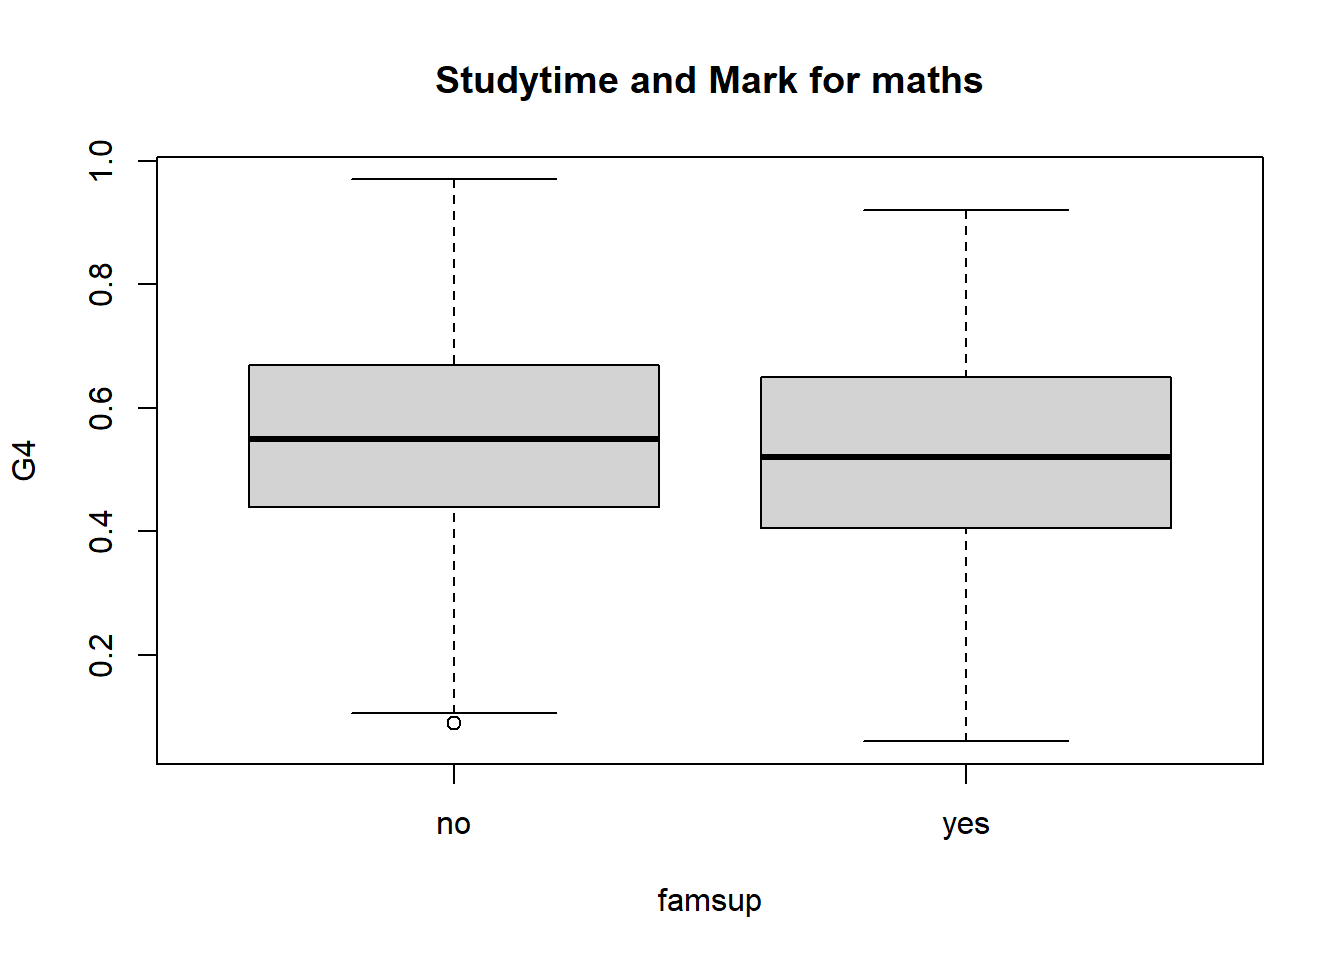
\includegraphics{journal-article_files/figure-latex/unnamed-chunk-7-1.pdf}

A similar trend appears when we compare student performance and their
frequency of social interactions, measured by the number of times they
go out per week. The cohort of students who report they ``go out'' at a
``low'' frequency attain the highest average grade surpassing all other
cohorts. This result may indicate that some form of social interaction
is necessary for a student to achieve a positive frame of mind needed to
excel academically. The caveat for this condition is too much ``going
out'' may detrimentally impact performance.

\hypertarget{alcohol}{%
\subsection{Alcohol}\label{alcohol}}

\begin{center}\rule{0.5\linewidth}{0.5pt}\end{center}

\begin{Shaded}
\begin{Highlighting}[]
\NormalTok{d.all <-}\StringTok{ }\NormalTok{d.all }\OperatorTok\StringTok{ }\KeywordTok{mutate}\NormalTok{(}\DataTypeTok{Walc =} \KeywordTok{case_when}\NormalTok{(}
\NormalTok{  Walc }\OperatorTok{==}\StringTok{ }\DecValTok{1} \OperatorTok{~}\StringTok{"Very Low"}\NormalTok{, }
\NormalTok{  Walc }\OperatorTok{==}\StringTok{ }\DecValTok{2} \OperatorTok{~}\StringTok{ "Low"}\NormalTok{, }
\NormalTok{  Walc }\OperatorTok{==}\StringTok{ }\DecValTok{3} \OperatorTok{~}\StringTok{ "Average"}\NormalTok{, }
\NormalTok{  Walc }\OperatorTok{==}\StringTok{ }\DecValTok{4} \OperatorTok{~}\StringTok{ "High"}\NormalTok{,}
\NormalTok{  Walc }\OperatorTok{==}\StringTok{ }\DecValTok{5} \OperatorTok{~}\StringTok{ "Very High"}
\NormalTok{))}


\NormalTok{d.all}\OperatorTok{$}\NormalTok{Walc =}\StringTok{ }\KeywordTok{factor}\NormalTok{(d.all}\OperatorTok{$}\NormalTok{Walc, }\DataTypeTok{levels =} \KeywordTok{c}\NormalTok{(}\StringTok{"Very Low"}\NormalTok{,}\StringTok{"Low"}\NormalTok{,}\StringTok{"Average"}\NormalTok{,}\StringTok{"High"}\NormalTok{,}\StringTok{'Very High'}\NormalTok{), }\DataTypeTok{ordered=}\OtherTok{TRUE}\NormalTok{)}

\NormalTok{d.all }\OperatorTok\StringTok{ }\KeywordTok{ggplot}\NormalTok{(}\KeywordTok{aes}\NormalTok{(}\DataTypeTok{x =}\NormalTok{ Walc, }\DataTypeTok{y =}\NormalTok{ G3)) }\OperatorTok{+}\StringTok{ }\KeywordTok{geom_boxplot}\NormalTok{() }\OperatorTok{+}\StringTok{ }\KeywordTok{labs}\NormalTok{(}\DataTypeTok{title =} \StringTok{"Academic performance by weekend alcohol consumption"}\NormalTok{, }\DataTypeTok{x =} \StringTok{""}\NormalTok{, }\DataTypeTok{y =} \StringTok{"Academic performance"}\NormalTok{) }\OperatorTok{+}\StringTok{ }\KeywordTok{theme_bw}\NormalTok{() }\OperatorTok{+}\StringTok{ }\KeywordTok{facet_wrap}\NormalTok{(}\OperatorTok{~}\StringTok{ }\NormalTok{subject, }\DataTypeTok{nrow =} \DecValTok{1}\NormalTok{)}
\end{Highlighting}
\end{Shaded}

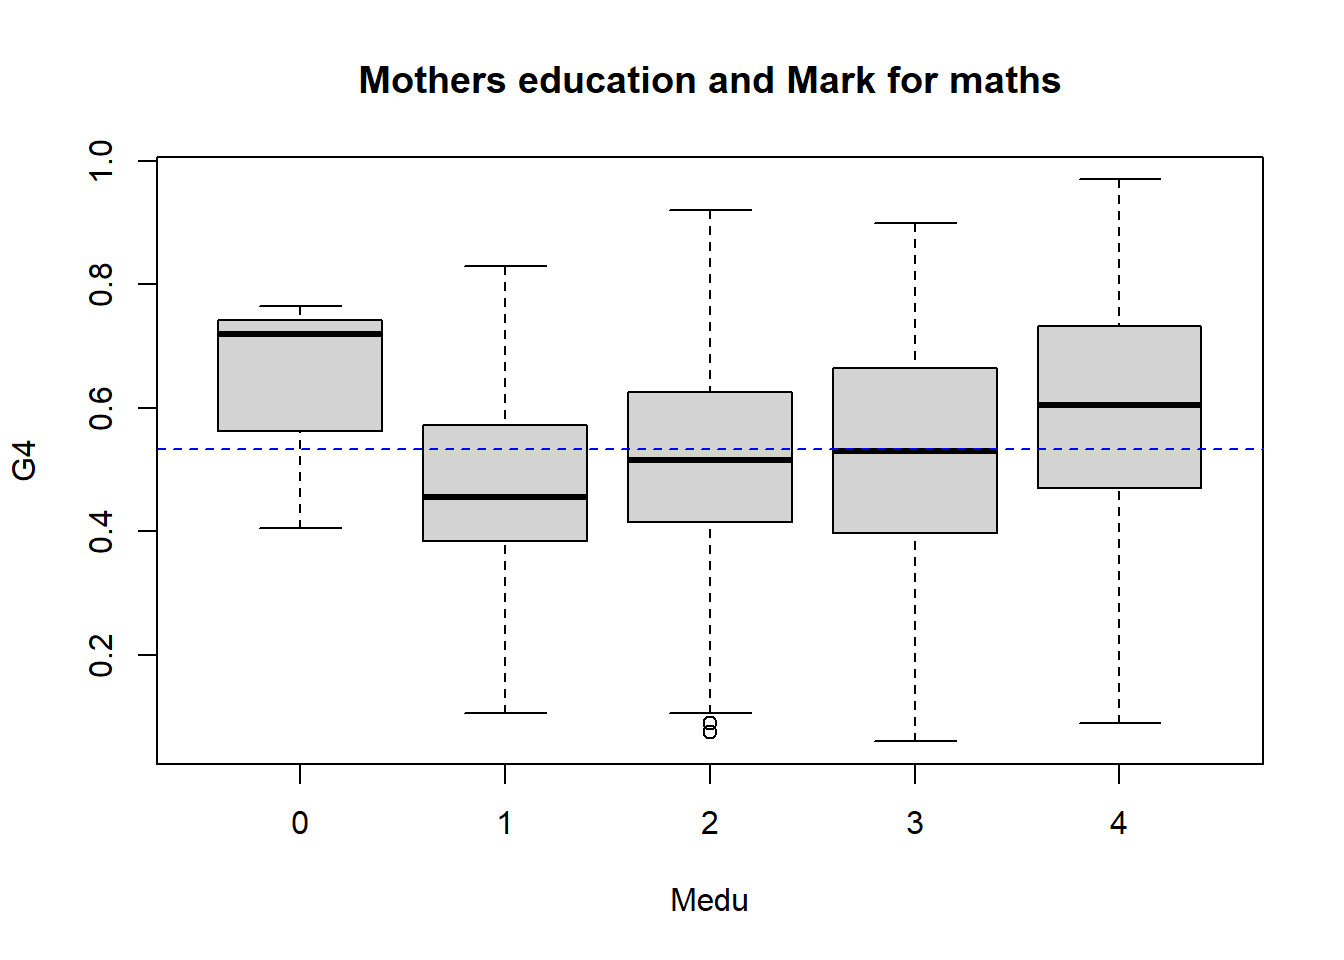
\includegraphics{journal-article_files/figure-latex/unnamed-chunk-8-1.pdf}

\hypertarget{but-mothers-education-matters-1}{%
\section{(but mother's education
matters)}\label{but-mothers-education-matters-1}}

\begin{center}\rule{0.5\linewidth}{0.5pt}\end{center}

\begin{Shaded}
\begin{Highlighting}[]
\NormalTok{d.all <-}\StringTok{ }\NormalTok{d.all }\OperatorTok\StringTok{ }\KeywordTok{mutate}\NormalTok{(}\DataTypeTok{Medu =} \KeywordTok{case_when}\NormalTok{(Medu }\OperatorTok{==}\StringTok{ }\DecValTok{0} \OperatorTok{~}\StringTok{ "None"}\NormalTok{,}
\NormalTok{                                  Medu }\OperatorTok{==}\StringTok{ }\DecValTok{1} \OperatorTok{~}\StringTok{ "4th Grade"}\NormalTok{, }
\NormalTok{                                  Medu }\OperatorTok{==}\StringTok{ }\DecValTok{2} \OperatorTok{~}\StringTok{ "5th - 9th Grade"}\NormalTok{, }
\NormalTok{                                  Medu }\OperatorTok{==}\StringTok{ }\DecValTok{3} \OperatorTok{~}\StringTok{ "Secondary Education"}\NormalTok{, }
\NormalTok{                                  Medu }\OperatorTok{==}\StringTok{ }\DecValTok{4} \OperatorTok{~}\StringTok{ "Higher Education"}\NormalTok{))}


\NormalTok{d.all}\OperatorTok{$}\NormalTok{Medu =}\StringTok{ }\KeywordTok{factor}\NormalTok{(d.all}\OperatorTok{$}\NormalTok{Medu, }\DataTypeTok{levels =}  \KeywordTok{c}\NormalTok{(}\StringTok{"None"}\NormalTok{, }\StringTok{"4th Grade"}\NormalTok{, }\StringTok{"5th - 9th Grade"}\NormalTok{,  }\StringTok{"Secondary Education"}\NormalTok{, }\StringTok{"Higher Education"}\NormalTok{), }\DataTypeTok{ordered =} \OtherTok{TRUE}\NormalTok{ )}
\CommentTok{#levels(d.all$Medu) = c("None", "4th Grade", "5th - 9th Grade",  "Secondary Education", "Higher #Education")}

\NormalTok{d.all }\OperatorTok\StringTok{ }
\StringTok{  }\KeywordTok{ggplot}\NormalTok{(}\KeywordTok{aes}\NormalTok{(}\DataTypeTok{x =}\NormalTok{ Medu, }\DataTypeTok{y =}\NormalTok{ G3, }\DataTypeTok{fill =}\NormalTok{ subject)) }\OperatorTok{+}\StringTok{ }\KeywordTok{geom_boxplot}\NormalTok{() }\OperatorTok{+}\StringTok{ }\KeywordTok{labs}\NormalTok{(}\DataTypeTok{title =} \StringTok{"Student performance by mother's education level"}\NormalTok{, }\DataTypeTok{x =} \StringTok{"Mother's education level"}\NormalTok{, }\DataTypeTok{y =} \StringTok{"Student performane"}\NormalTok{, }\DataTypeTok{fill =} \StringTok{"Subject"}\NormalTok{) }\OperatorTok{+}\StringTok{ }\KeywordTok{theme_bw}\NormalTok{() }\OperatorTok{+}\StringTok{ }\KeywordTok{theme}\NormalTok{(}\DataTypeTok{axis.text.x =} \KeywordTok{element_text}\NormalTok{(}\DataTypeTok{angle =} \DecValTok{45}\NormalTok{, }\DataTypeTok{hjust=}\DecValTok{1}\NormalTok{))}
\end{Highlighting}
\end{Shaded}

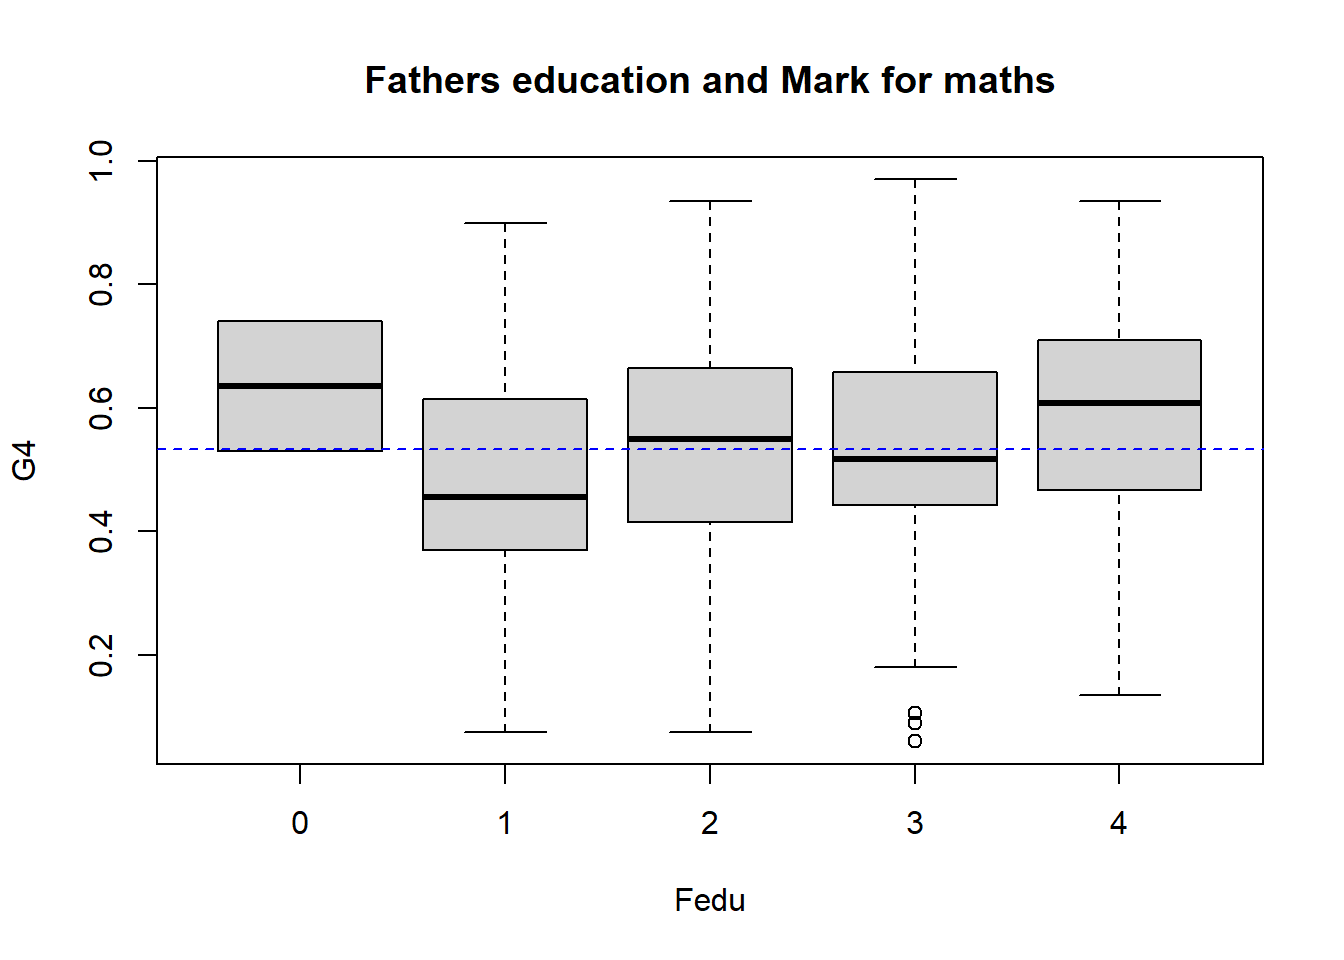
\includegraphics{journal-article_files/figure-latex/unnamed-chunk-9-1.pdf}

In this study, a student's mark in both Portugese and Math increased
positively with his mother's and father's education level. As shown in
the figure above, when mothers have a low education level, their
children perform poorly compared to their peers. One study in 2015
explored how parent-education levels affected student engagement in
school over a period of several years in Japan (Matsuoka et al., 2015).
They found that a parent's education level influenced their parenting
style: highly-educated parents tend to schedule their children's time
with more extracurricular activities, and place a larger emphasis on
engaging language to reason. Educated parents may also have higher
expectations for their children's academic achievement, which could
subsequently influence their desires to pursue higher education: one
study found that the mother's expectations for her children had an
impact on whether they wanted to attend university (Uzuki, 2004).

\begin{Shaded}
\begin{Highlighting}[]
\NormalTok{d.all }\OperatorTok\StringTok{ }\KeywordTok{ggplot}\NormalTok{(}\KeywordTok{aes}\NormalTok{(}\DataTypeTok{x =}\NormalTok{ Medu, }\DataTypeTok{y =}\NormalTok{ G3, }\DataTypeTok{fill =}\NormalTok{ studytime)) }\OperatorTok{+}\StringTok{ }\KeywordTok{geom_boxplot}\NormalTok{() }\OperatorTok{+}\StringTok{ }\KeywordTok{labs}\NormalTok{(}\DataTypeTok{title =} \StringTok{"Student performance by mother's education level"}\NormalTok{, }\DataTypeTok{x =} \StringTok{"Mother's education level"}\NormalTok{, }\DataTypeTok{y =} \StringTok{"Student performane"}\NormalTok{, }\DataTypeTok{fill =} \StringTok{"Study time (hours)"}\NormalTok{) }\OperatorTok{+}\StringTok{ }\KeywordTok{theme_bw}\NormalTok{() }\OperatorTok{+}\StringTok{ }\KeywordTok{facet_wrap}\NormalTok{(}\OperatorTok{~}\NormalTok{subject, }\DataTypeTok{nrow =} \DecValTok{2}\NormalTok{) }\OperatorTok{+}\StringTok{ }\KeywordTok{theme}\NormalTok{(}\DataTypeTok{axis.text.x =} \KeywordTok{element_text}\NormalTok{(}\DataTypeTok{angle =} \DecValTok{45}\NormalTok{, }\DataTypeTok{hjust=}\DecValTok{1}\NormalTok{))}
\end{Highlighting}
\end{Shaded}

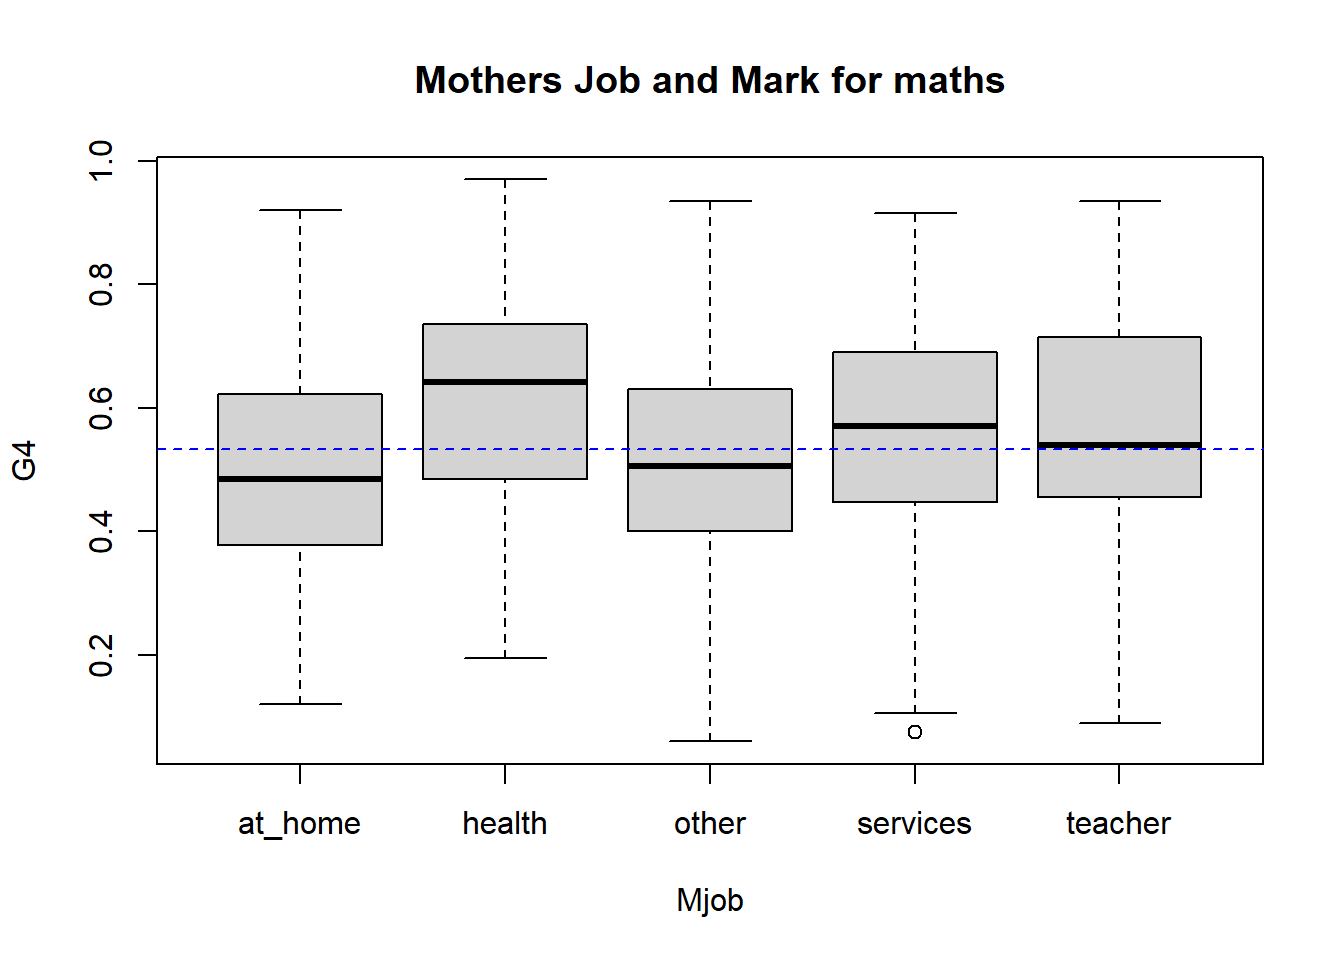
\includegraphics{journal-article_files/figure-latex/unnamed-chunk-10-1.pdf}

Although parent education appears to affect how students spend their
free time and shape their future academic goals, individual effort
appears to pay off more for students from poorly-educated families. The
above figure shows there was a larger increase in sacacemic achievement
per increase in hours studies for students with poorly-educated mothers
compared to students with highly educated mothers.

\hypertarget{student-choices-on-student-achievement-1}{%
\section{Student choices on student
achievement}\label{student-choices-on-student-achievement-1}}

\begin{center}\rule{0.5\linewidth}{0.5pt}\end{center}

\begin{Shaded}
\begin{Highlighting}[]
\NormalTok{d.all <-}\StringTok{ }\NormalTok{d.all }\OperatorTok\StringTok{ }\KeywordTok{mutate}\NormalTok{(}\DataTypeTok{goout =} \KeywordTok{case_when}\NormalTok{(}
\NormalTok{  goout }\OperatorTok{==}\StringTok{ }\DecValTok{1} \OperatorTok{~}\StringTok{"Very Low"}\NormalTok{, }
\NormalTok{  goout }\OperatorTok{==}\StringTok{ }\DecValTok{2} \OperatorTok{~}\StringTok{ "Low"}\NormalTok{, }
\NormalTok{  goout }\OperatorTok{==}\StringTok{ }\DecValTok{3} \OperatorTok{~}\StringTok{ "Average"}\NormalTok{, }
\NormalTok{  goout }\OperatorTok{==}\StringTok{ }\DecValTok{4} \OperatorTok{~}\StringTok{ "High"}\NormalTok{,}
\NormalTok{  goout }\OperatorTok{==}\StringTok{ }\DecValTok{5} \OperatorTok{~}\StringTok{ "Very High"}
\NormalTok{))}

\NormalTok{d.all}\OperatorTok{$}\NormalTok{goout =}\StringTok{ }\KeywordTok{factor}\NormalTok{(d.all}\OperatorTok{$}\NormalTok{goout, }\DataTypeTok{levels =} \KeywordTok{c}\NormalTok{(}\StringTok{"Very Low"}\NormalTok{,}\StringTok{"Low"}\NormalTok{,}\StringTok{"Average"}\NormalTok{,}\StringTok{"High"}\NormalTok{,}\StringTok{'Very High'}\NormalTok{), }\DataTypeTok{ordered=}\OtherTok{TRUE}\NormalTok{)}

\NormalTok{d.all }\OperatorTok\StringTok{ }\KeywordTok{ggplot}\NormalTok{(}\KeywordTok{aes}\NormalTok{(}\DataTypeTok{x =}\NormalTok{ goout, }\DataTypeTok{y =}\NormalTok{ G3)) }\OperatorTok{+}\StringTok{ }\KeywordTok{geom_boxplot}\NormalTok{() }\OperatorTok{+}\StringTok{ }\KeywordTok{labs}\NormalTok{(}\DataTypeTok{title =} \StringTok{"Academic performance by time spent going out with friends"}\NormalTok{, }\DataTypeTok{x =} \StringTok{""}\NormalTok{, }\DataTypeTok{y =} \StringTok{"Academic performance"}\NormalTok{) }\OperatorTok{+}\StringTok{ }\KeywordTok{theme_bw}\NormalTok{() }\OperatorTok{+}\StringTok{ }\KeywordTok{facet_wrap}\NormalTok{(}\OperatorTok{~}\StringTok{ }\NormalTok{subject, }\DataTypeTok{nrow =} \DecValTok{1}\NormalTok{)}
\end{Highlighting}
\end{Shaded}

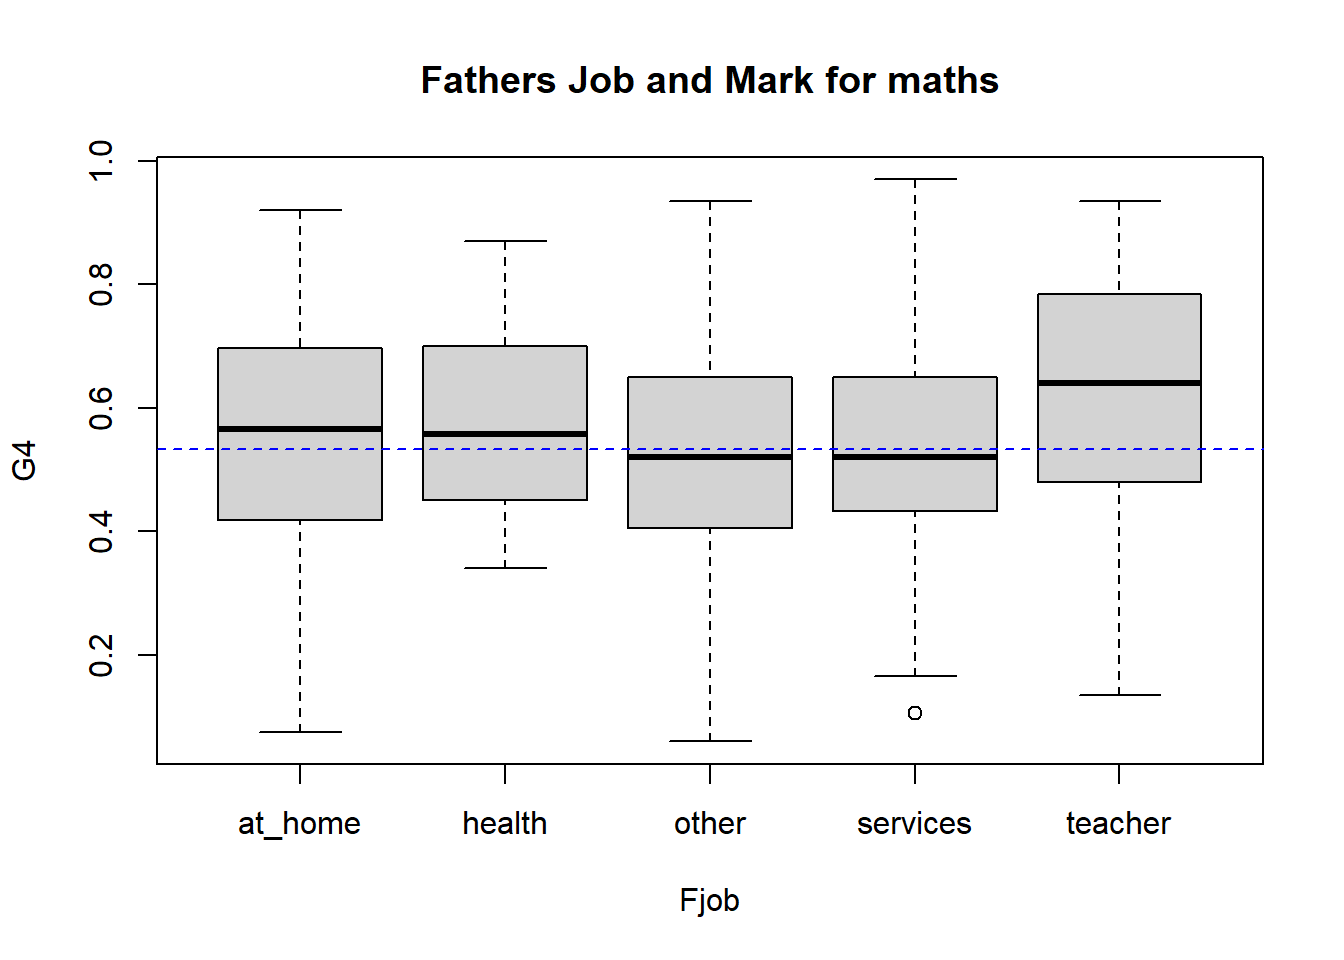
\includegraphics{journal-article_files/figure-latex/unnamed-chunk-11-1.pdf}

\begin{Shaded}
\begin{Highlighting}[]
\NormalTok{d.all <-}\StringTok{ }\NormalTok{d.all }\OperatorTok\StringTok{ }\KeywordTok{mutate}\NormalTok{(}\DataTypeTok{Walc =} \KeywordTok{case_when}\NormalTok{(}
\NormalTok{  Walc }\OperatorTok{==}\StringTok{ }\DecValTok{1} \OperatorTok{~}\StringTok{"Very Low"}\NormalTok{, }
\NormalTok{  Walc }\OperatorTok{==}\StringTok{ }\DecValTok{2} \OperatorTok{~}\StringTok{ "Low"}\NormalTok{, }
\NormalTok{  Walc }\OperatorTok{==}\StringTok{ }\DecValTok{3} \OperatorTok{~}\StringTok{ "Average"}\NormalTok{, }
\NormalTok{  Walc }\OperatorTok{==}\StringTok{ }\DecValTok{4} \OperatorTok{~}\StringTok{ "High"}\NormalTok{,}
\NormalTok{  Walc }\OperatorTok{==}\StringTok{ }\DecValTok{5} \OperatorTok{~}\StringTok{ "Very High"}
\NormalTok{))}



\NormalTok{d.all }\OperatorTok\StringTok{ }\KeywordTok{ggplot}\NormalTok{(}\KeywordTok{aes}\NormalTok{(}\DataTypeTok{x =}\NormalTok{ Walc, }\DataTypeTok{y =}\NormalTok{ G3)) }\OperatorTok{+}\StringTok{ }\KeywordTok{geom_boxplot}\NormalTok{() }\OperatorTok{+}\StringTok{ }\KeywordTok{labs}\NormalTok{(}\DataTypeTok{title =} \StringTok{"Academic performance by weekend alcohol consumption"}\NormalTok{, }\DataTypeTok{x =} \StringTok{""}\NormalTok{, }\DataTypeTok{y =} \StringTok{"Academic performance"}\NormalTok{) }\OperatorTok{+}\StringTok{ }\KeywordTok{theme_bw}\NormalTok{() }\OperatorTok{+}\StringTok{ }\KeywordTok{facet_wrap}\NormalTok{(}\OperatorTok{~}\StringTok{ }\NormalTok{subject, }\DataTypeTok{nrow =} \DecValTok{1}\NormalTok{)}
\end{Highlighting}
\end{Shaded}

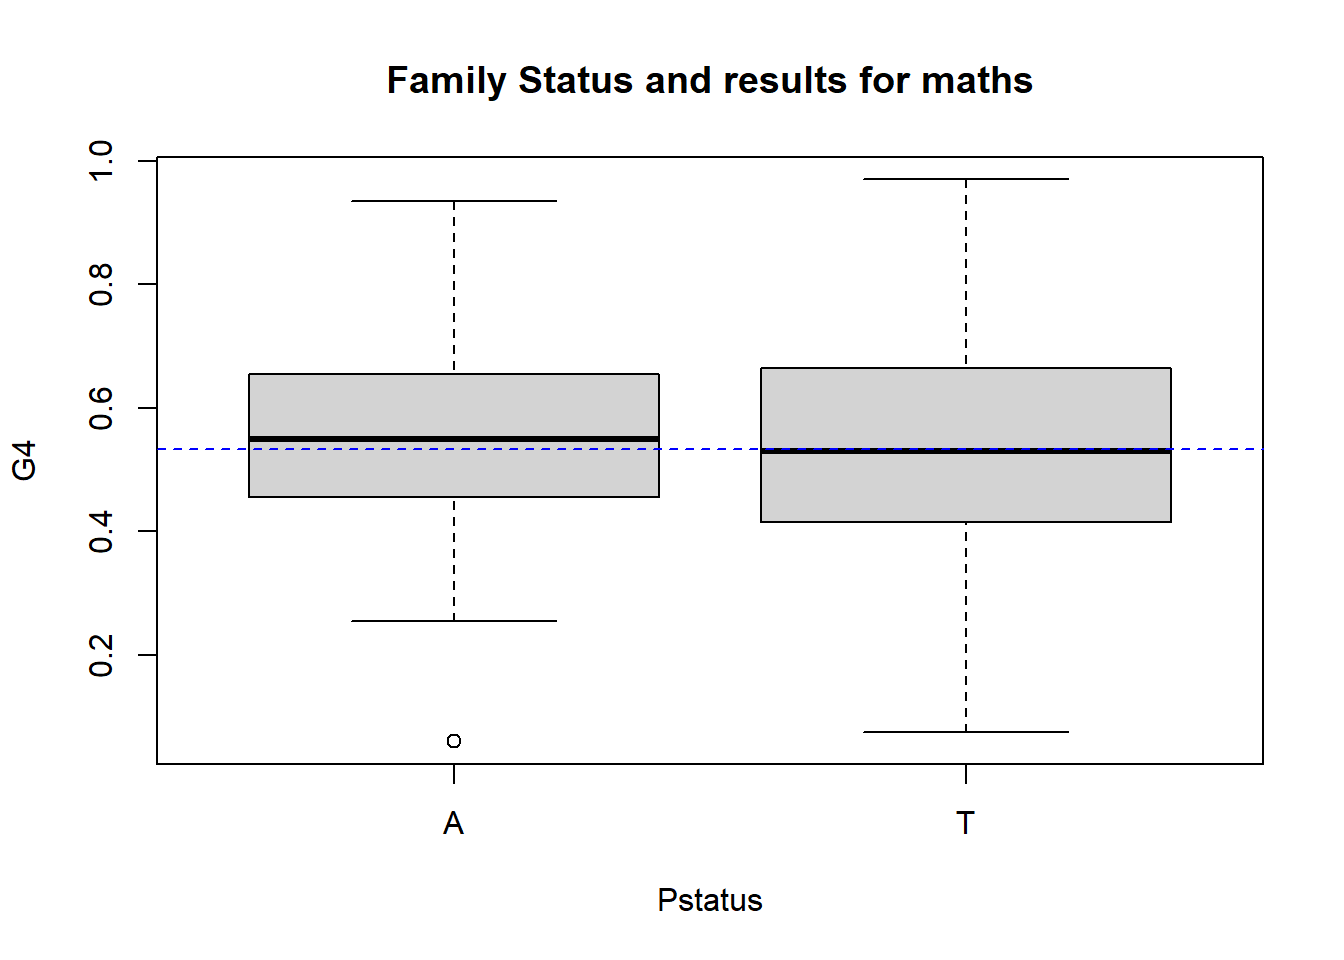
\includegraphics{journal-article_files/figure-latex/unnamed-chunk-12-1.pdf}

\begin{Shaded}
\begin{Highlighting}[]
\NormalTok{d.all <-}\StringTok{ }\NormalTok{d.all }\OperatorTok\StringTok{ }\KeywordTok{mutate}\NormalTok{(}\DataTypeTok{freetime =} \KeywordTok{case_when}\NormalTok{(}
\NormalTok{  freetime }\OperatorTok{==}\StringTok{ }\DecValTok{1} \OperatorTok{~}\StringTok{"Very Low"}\NormalTok{, }
\NormalTok{  freetime }\OperatorTok{==}\StringTok{ }\DecValTok{2} \OperatorTok{~}\StringTok{ "Low"}\NormalTok{, }
\NormalTok{  freetime }\OperatorTok{==}\StringTok{ }\DecValTok{3} \OperatorTok{~}\StringTok{ "Average"}\NormalTok{, }
\NormalTok{  freetime }\OperatorTok{==}\StringTok{ }\DecValTok{4} \OperatorTok{~}\StringTok{ "High"}\NormalTok{,}
\NormalTok{  freetime }\OperatorTok{==}\StringTok{ }\DecValTok{5} \OperatorTok{~}\StringTok{ "Very High"}
\NormalTok{))}

\NormalTok{d.all }\OperatorTok\StringTok{ }\KeywordTok{ggplot}\NormalTok{(}\KeywordTok{aes}\NormalTok{(}\DataTypeTok{x =}\NormalTok{ Walc, }\DataTypeTok{y =}\NormalTok{ G3)) }\OperatorTok{+}\StringTok{ }\KeywordTok{geom_boxplot}\NormalTok{() }\OperatorTok{+}\StringTok{ }\KeywordTok{labs}\NormalTok{(}\DataTypeTok{title =} \StringTok{"Academic performance by free time after school"}\NormalTok{, }\DataTypeTok{x =} \StringTok{""}\NormalTok{, }\DataTypeTok{y =} \StringTok{"Academic performance"}\NormalTok{) }\OperatorTok{+}\StringTok{ }\KeywordTok{theme_bw}\NormalTok{() }\OperatorTok{+}\StringTok{ }\KeywordTok{facet_wrap}\NormalTok{(}\OperatorTok{~}\StringTok{ }\NormalTok{subject, }\DataTypeTok{nrow =} \DecValTok{1}\NormalTok{)}
\end{Highlighting}
\end{Shaded}

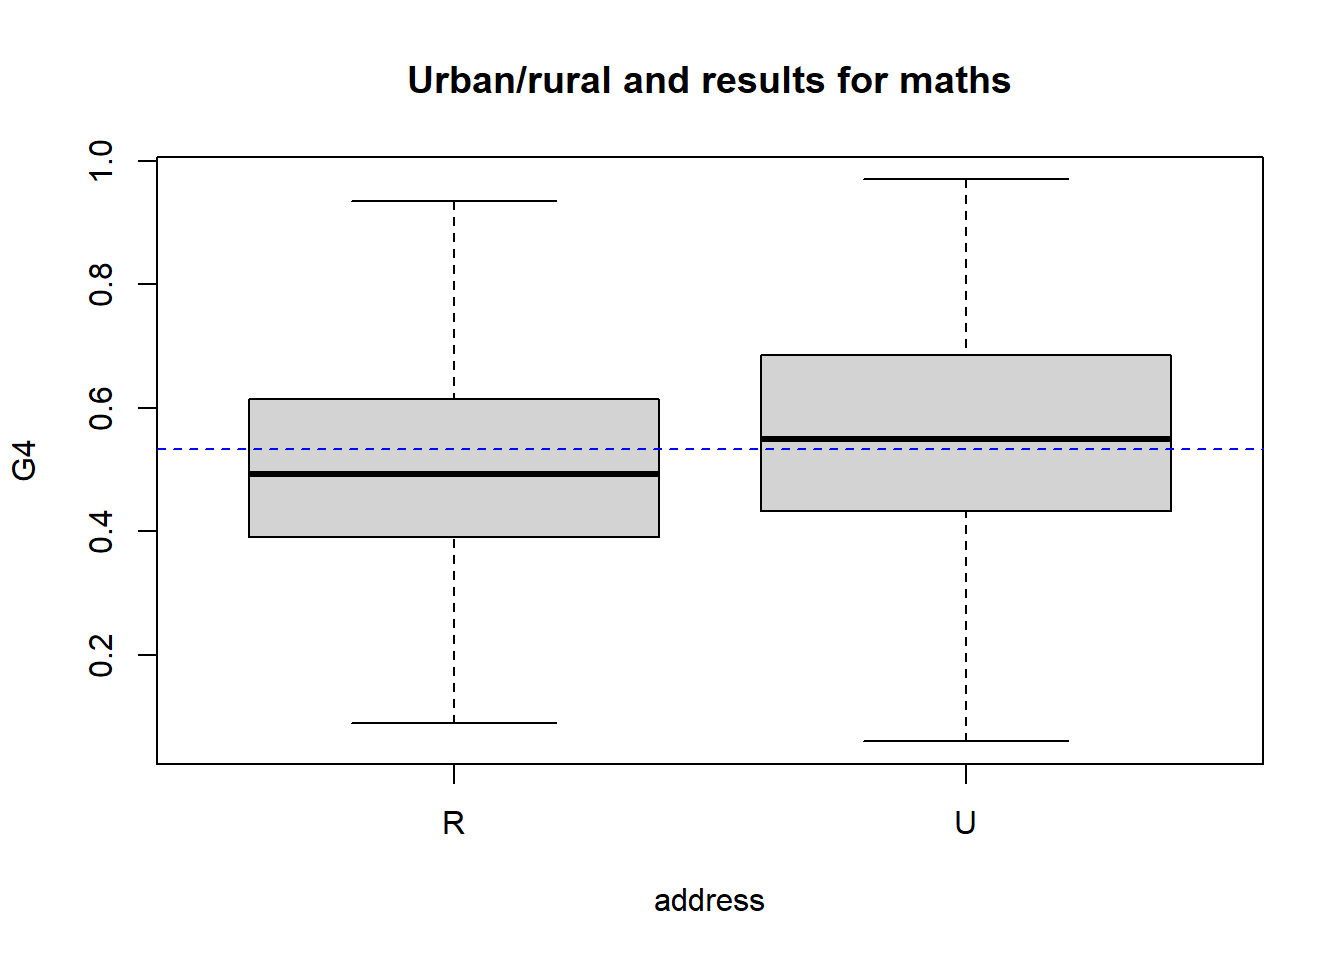
\includegraphics{journal-article_files/figure-latex/unnamed-chunk-13-1.pdf}

\hypertarget{conclusion}{%
\section{Conclusion}\label{conclusion}}

References

\begin{itemize}
\tightlist
\item
  Matsuoka, R., Nakamuro, M. and Inui, T., 2015. Emerging inequality in
  effort: A longitudinal investigation of parental involvement and early
  elementary school-aged children's learning time in Japan. Social
  Science Research, 54, pp.159-176.
\end{itemize}

\end{document}
